\documentclass[10pt,a4paper, margin=1in]{article}
\usepackage{fullpage}
\usepackage{amsfonts, amsmath, pifont}
\usepackage{amsthm}
\usepackage{graphicx}
\usepackage{float}

\usepackage{tkz-euclide}
\usepackage{tikz}
\usepackage{pgfplots}
\pgfplotsset{compat=1.13}

\usepackage{geometry}
 \geometry{
 a4paper,
 total={210mm,297mm},
 left=10mm,
 right=10mm,
 top=10mm,
 bottom=10mm,
 }
 % Write both of your names here. Fill exxxxxxx with your ceng mail address.
 \author{
  Deveci, Cengizhan\\
  \texttt{e2448322@ceng.metu.edu.tr}
  \and
  İşleyici, Osman Taylan\\
  \texttt{e2448496@ceng.metu.edu.tr}
}

\title{CENG 384 - Signals and Systems for Computer Engineers \\
Spring 2023 \\
Homework 2}
\begin{document}
\maketitle



\noindent\rule{19cm}{1.2pt}

\begin{enumerate}

\item %write the solution of q1
    \begin{enumerate}
    % Write your solutions in the following items.
    \item $\int x(t) - 5 y(t) dt = y(t)$\\
    If we differentiate both sides;\\
    $x(t) - 5y(t) = y'(t)$\\
    \item %write the solution of q1b
    Since the system is linear,\\
    $y_p(t) = K_1e^{-t}u(t) + K_2e^{-3t}u(t)$\\
    For the first term;\\
    $e^{-t}u(t) = (-K_1 + 5K_1)e^{-t}u(t)$\\
    $K_1 = \frac{1}{4}$\\
    Similarly;\\
    $-3K_2 + 5K_2 = 1$\\
    $K_2 = \frac{1}{2}$\\
    $y_p(t) = \frac{1}{4}e^{-t}u(t) + \frac{1}{2}e^{-3t}u(t)$\\
    $y_h(t) = Ce^{\alpha t}$\\
    $y_h'(t) = \alpha C e^{\alpha t}$\\
    $\alpha C + 5 C = 0$\\
    $\alpha = -5$\\
    $y(t) = \frac{1}{4}e^{-t}u(t) + \frac{1}{2}e^{-3t}u(t) - \frac{3}{4}e^{-5t}$\\
    (Since $y(0) = 0, C = -3/4$).\\
    \end{enumerate}

\item %write the solution of q2  
	\begin{enumerate}
    % Write your solutions in the following items.
    \item %write the solution of q2a
    $x[n] = 2 \delta [n] + \delta [n+1], h[n] = \delta[n-1]+2\delta[n+1]$\\

    $y[n] = x[n] * h[n] = \sum_{k=-\infty}^{\infty}x[k]h[n-k]$ \\

    $= \sum_{k=-\infty}^{\infty}2\delta[k]\delta[n-k-1] + \sum_{k=-\infty}^{\infty}\delta[k + 1]\delta[n-k-1] + \sum_{k=-\infty}^{\infty}2\delta[k]2\delta[n-k+1] + \sum_{k=-\infty}^{\infty}\delta[k + 1]\delta[n-k+1]$ \\

    $y[n] = 2\delta[n - 1] + \delta[n] + 4\delta[n+1] + 2\delta[n+2]$ \\

    \begin{filecontents}{data2a.dat}
        n   xn
        -3   0
        -2   2
        -1   4
        0    1
        1    2
        2    0
       \end{filecontents}

       \begin{tikzpicture}
         \begin{axis}[
             axis lines=middle,
             xlabel={$n$},
             ylabel={$\boldsymbol{y[n]}$},
             ytick={0, 1, ..., 5},
             xtick={-3, -2, ..., 2},
             enlarge x limits={abs=1},
             ymin=0, ymax=5,
             xticklabel style={
               fill=white,
               fill opacity=0.7,
               text opacity=1,
               inner sep=1pt,
             },
             axis on top,
           ]
           \addplot [ycomb, black, thick, mark=*] table [x={n}, y={xn}] {data2a.dat};
         \end{axis}
       \end{tikzpicture}
    
    \item %write the solution of q2b
    $x(t) = u(t-1) + u(t+1), h[t] = e^{-t}sin(t)u(t), y(t) = \frac{dx(t)}{dt}*h(t)$\\

    $\dot{x}(t) = \delta(t-1)+\delta(t+1)$ \\

    $y(t) = \dot{x}(t) * h(t)$ \\

    $(\delta(t-1)*h(t)) + (\delta(t+1)*h(t))$ \\

    $=h(t - 1) + h(t + 1)$ \\

    $y(t) = e^{-(t-1)}sin(t-1)u(t-1) + e^{-(t+1)} sin(t+1)u(t+1)$
    \end{enumerate}

\item %write the solution of q3
    \begin{enumerate}
    % Write your solutions in the following items.
    \item $\int_{-\inf}^{\inf} h(\tau)x(t-\tau)d\tau$\\
    $\int_{-\inf}^{\inf} e^{-2\tau}u(\tau)e^{-t+\tau}u(t-\tau)d\tau$\\
    $\int_{-\inf}^{\inf} e^{-\tau-t}u(\tau)u(t-\tau)d\tau$\\
    Since $u(t-\tau)$ is 0 except $\tau <= t$;\\
    $\int_0^t e^{-t-\tau} d\tau$\\
    $e^{-t}*(e^{-t}+1) = e^{-2t} + e^{-t}$\\
    \item %write the solution of q3b
    $\int_{-\inf}^{\inf} e^{3t-3\tau}u(t-\tau)u(\tau)dt - \int_{-\inf}^{\inf}e^{3t-3\tau}u(t-\tau)u(\tau-1)$\\
    First part of equation;\\
    $\int^t_1 e^{3t}e^{-3\tau}dt = -e^{3t} + \frac{1}{3}$\\
    Second part of equation;\\
    $e^[3t]\int^t_1 e^{-3\tau} dt = -1 + e^{3t-3}$\\
    $-\frac{2}{3} + e^{3t-3} + -e^{3t}$\\
    \end{enumerate}

\item %write the solution of q4
    \begin{enumerate}   
    % Write your solutions in the following items.
    \item %write the solution of q4a
    Let's write the characteristic equation, \\

    $\lambda^2 -\lambda-1 = 0$ \\

    $\Delta = 1 + 4 = 5$ \\

    $\lambda_1 = \frac{1}{2}(1+\sqrt{5})$ \\

    $\lambda_2 = \frac{1}{2}(1-\sqrt{5})$ \\

    $y[n] = A(\frac{1}{2}(1+\sqrt{5}))^n + B (\frac{1}{2}(1-sqrt{5}))^n$\\

    For initial conditions: \\

    $y[0] = 1 => A + B = 1$ \\

    $y[1] = 1 => A(\frac{1+\sqrt{5}}{2}) + B(\frac{1-\sqrt{5}}{2})$ \\

    Multiple by $\frac{-\sqrt{5} - 1}{2}$ and sum both part. \\

    $-B = \frac{1-\sqrt{5}}{2} => B = \frac{\sqrt{5} - 1}{2}$ \\

    $A = 1 - B = 1 - \frac{\sqrt{5} - 1}{2} = \frac{3 - \sqrt{5}}{2}$

    $y[n] = (\frac{3 - \sqrt{5}}{2})(\frac{1}{2}(1+\sqrt{5}))^n + (\frac{\sqrt{5} - 1}{2}) (\frac{1}{2}(1-sqrt{5}))^n$\\
    \item %write the solution of q4b
    Let's write the characteristic equation, \\

    $\lambda^2-6\lambda^2+13\lambda-10 = 0$\\

    $(\lambda-2)(\lambda^2-4\lambda+5) = (\lambda-2)(\lambda - (2 - i))(\lambda - (2 + i))$ \\

    $y(t) = Ae^{2t}+Be^{(2-i)t}+Ce^{(2-i)t}$\\

    $y(0) = A + B + C = 1$ \\

    $y'(0) = 2A + (2-i)B + (2+i)C = \frac{3}{2}$\\

    $y''(0) = 4A + (2-i)^2B+(2+i)^2C = 3$ \\

    $i(-B+C) = -\frac{1}{2}$\\

    $A = -2 => B + C = 3$ \\

    Then $B = \frac{6 - i}{4}$ \\

    $C = \frac{6 + i}{4}$\\

    As a result $y(t) = -2e^{2t}+(\frac{6 - i}{4})e^{(2-i)t}+(\frac{6 + i}{4})e^{(2-i)t}$
    \end{enumerate}

\item %write the solution of q5
    \begin{enumerate}
    % Write your solutions in the following items.
    \item 
    $cos(5t) = \frac{e^{5it} + e^{-5it}}{2}$\\
    $y_{p1} = ke^{5it}/2$\\
    $y_{p1}' = 5ike^{5it}/2$\\
    $y_{p1}'' = -25ke^{5it}/2$\\
    $-25k+25ik+6k = 1$\\
    $k_1=\frac{-19}{986} + \frac{-25i}{986}$\\
    $y_{p2} = k_2e^{-5it}/2$\\
    $y_{p2}' = -5i k_2e^{-5it}/2$\\
    $y_{p2}'' = -25k_2e^{-5it}/2$\\
    $-19k_2 - 25k_2 = 1$\\
    $k_2 = \frac{-19 +25i}{986}$\\
    \item %write the solution of q5b
    $y_h(t) = Ce^{\alpha t}$\\
    $\alpha^2 + 5\alpha+6=0$\\
    $\alpha = -3 V -2$\\
    $y_h(t) = C(e^{-3t} + Ce^{-2t})$\\
	\item %write the solution of q5c
	$y(0) = 0 => \frac{-38}{986} + C = 0 $\\
    $y(t) = \frac{-19 - 25i}{986}e^{5it}/2 + \frac{25i-19}{986}e^{-5it}/2 + \frac{38(e^{-3t} + e^{-2t})}{986}$\\
    \end{enumerate}    
    
\item %write the solution of q6
    \begin{enumerate}
    % Write your solutions in the following items.
    \item %write the solution of q6a
    $x[n] * h_0[n] = w[n]$ \\

    say $x[n] = \delta[n]$\\

    $\delta[n] * h_0[n] = w[n] => h_0[n] = w[n]$ \\

    $h_0[n] - \dfrac{1}{2}h_0[n-1] = \delta[n]$ \\

    System is rest so $h_0[n] = 0$ for $n < 0$ and $\delta[n] = 1$ for n = 0, otherwise zero.

    $h_0[n] = \delta[n] + \frac{1}{2}h_0[n-1]$ \\

    $h_0[0] = 1 + 0$ \\

    $h_0[1] = 0 + \frac{1}{2}$ \\ 

    $h_0[2] = 0 + \frac{1}{4}$ \\ 

    $h_0[3] = 0 + \frac{1}{8}$ \\

    So $h_0[n] = \frac{1}{2^n}u[n]$
    \item %write the solution of q6b
    $h[n] = h_0[n] * h_0[n]$ \\

    $\sum_{k=-\infty}^{\infty}h_0[k]h_0[n-k] = \sum_{k=-\infty}^{\infty}\frac{1}{2^k}u[k]\frac{1}{2^{n-k}}u[n-k]$ \\

    for $k < 0, u[k] = 0$ and for $ k > n, u[n-k] = 0$ so we can set the border of the summation accordingly.\\

    $h[n] = \sum_{k=0}^{n}\frac{1}{2^n} = \frac{n}{2^n}$\\

	\item %write the solution of q6c
	We can write $y[n] - \frac{1}{2}y[n-1]=w[n]$ from second conv.\\

    We are trying to get $w[n] - \frac{1}{2}w[n-1]$ since it equals $x[n]$\\

    $y[n] - \frac{1}{2}y[n-1]=w[n]$ \\

    $-\frac{1}{2}(y[n-1] - \frac{1}{2}y[n-2])=-\frac{1}{2}w[n-1]$ \\

    $y[n] - y[n-1] +\frac{1}{4} y[n-2] = w[n] - \frac{1}{2}w[n-1]$ \\

    $y[n] - y[n-1] +\frac{1}{4} y[n-2] = x[n]$ \\
    \end{enumerate}
    
\item %write the solution of q7
    \begin{enumerate}
    % Write your solutions in the following items.
    \item~\\
    \begin{figure}[H]
        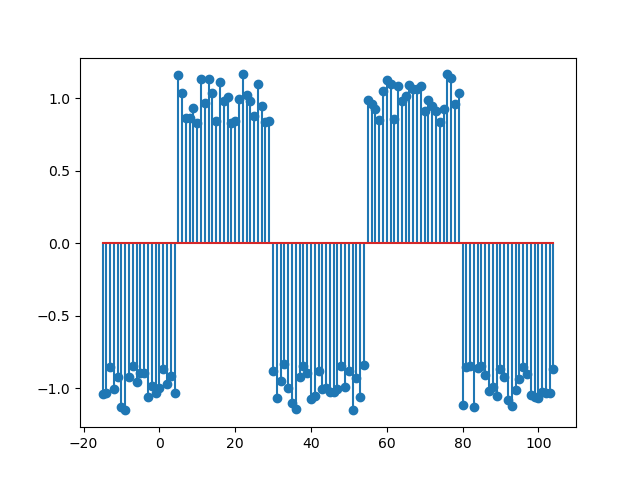
\includegraphics[scale = 0.75]{7_a.png}
    \end{figure}
    We can see that the result is actually equal to y(t-5). So convolving with impulse function results in delay.\\
    \item ~\\
    \begin{figure}[H]
        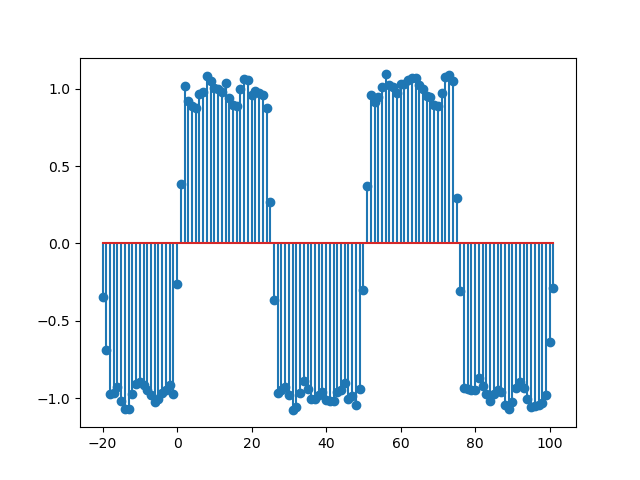
\includegraphics[scale=0.75]{7_b1.png}
        \caption{N=3}
    \end{figure}
    \begin{figure}[H]
        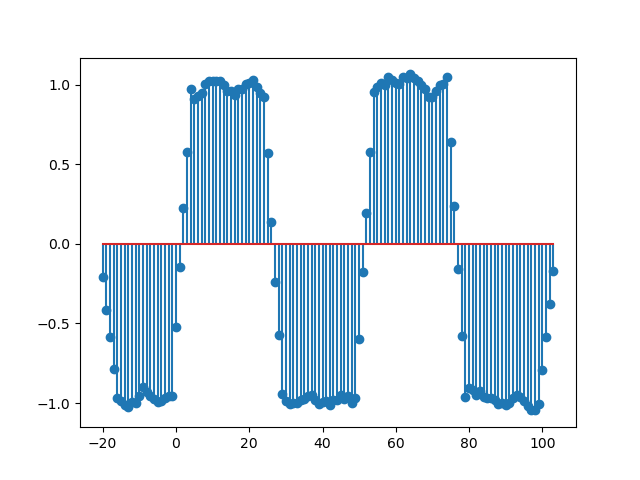
\includegraphics[scale=0.75]{7b_2.png}
        \caption{N=5}
    \end{figure}
    \begin{figure}[H]
        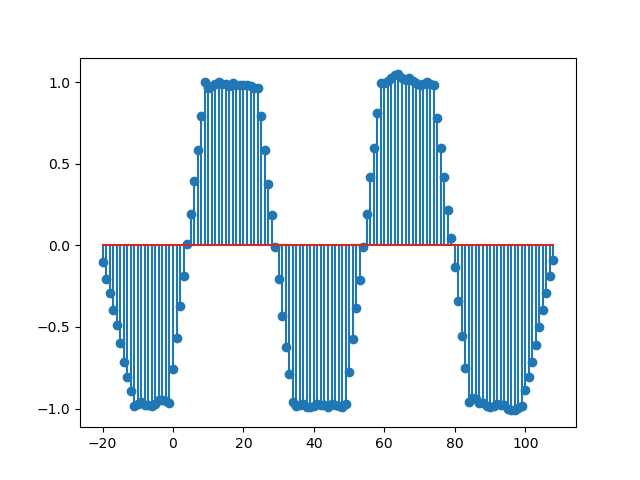
\includegraphics[scale=0.75]{7b_3.png}
        \caption{N=10}
    \end{figure}
    \begin{figure}[H]
        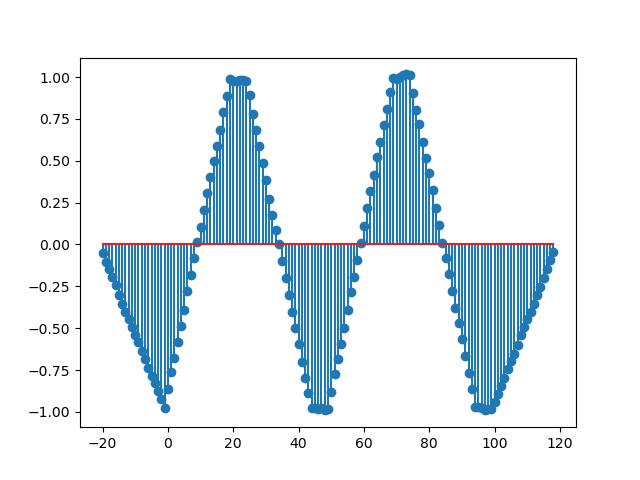
\includegraphics[scale=0.75]{7b_4.png}
        \caption{N=10}
    \end{figure}
    We can see that for larger values of N the graph diverges from our original graph because moving average change more significantly in less N values.
    \end{enumerate}    

\end{enumerate}


\end{document}

